\documentclass{article}

\usepackage[utf8]{inputenc}
\usepackage{titlesec}
\usepackage{easylist}
\usepackage{hanging}
\usepackage{hyperref}
\usepackage[a4paper,top=2.0cm,bottom=2.0cm,left=2.0cm,right=2.0cm]{geometry}
\usepackage{blindtext}
\usepackage{tipa}
\usepackage{epigraph}
\usepackage{enumerate}
\usepackage{longtable}
\usepackage{setspace}
\usepackage{verbatim}
\usepackage[T1]{fontenc}
\usepackage{graphicx}
\usepackage[italian]{babel}
\usepackage{amsmath}
\usepackage{pbox}
\usepackage{fancyhdr}
\usepackage{cancel}
\usepackage{tabularx}
\usepackage{booktabs}
\usepackage{multirow}
\usepackage{longtable}
\usepackage{tikz}
\usepackage{tikz-qtree}
\usepackage{subfig}
\usepackage{xcolor}
\usepackage{amssymb}
\usepackage{mathrsfs}
\usepackage{textcomp}
\usepackage{tasks}
\usepackage{upgreek}
\usepackage{listings}
\usepackage{color}

\definecolor{mygreen}{rgb}{0,0.6,0}
\definecolor{mygray}{rgb}{0.5,0.5,0.5}
\definecolor{mymauve}{rgb}{0.58,0,0.82}

\lstset{ 
  backgroundcolor=\color{white},   % choose the background color; you must add \usepackage{color} or \usepackage{xcolor}; should come as last argument
  basicstyle=\footnotesize,        % the size of the fonts that are used for the code
  breakatwhitespace=false,         % sets if automatic breaks should only happen at whitespace
  breaklines=true,                 % sets automatic line breaking
  captionpos=b,                    % sets the caption-position to bottom
  commentstyle=\color{mygreen},    % comment style
  deletekeywords={...},            % if you want to delete keywords from the given language
  escapeinside={\%*}{*)},          % if you want to add LaTeX within your code
  extendedchars=true,              % lets you use non-ASCII characters; for 8-bits encodings only, does not work with UTF-8
  firstnumber=1000,                % start line enumeration with line 1000
  frame=single,	                   % adds a frame around the code
  keepspaces=true,                 % keeps spaces in text, useful for keeping indentation of code (possibly needs columns=flexible)
  keywordstyle=\color{blue},       % keyword style
  language=Octave,                 % the language of the code
  morekeywords={*,...},            % if you want to add more keywords to the set
  numbers=left,                    % where to put the line-numbers; possible values are (none, left, right)
  numbersep=5pt,                   % how far the line-numbers are from the code
  numberstyle=\tiny\color{mygray}, % the style that is used for the line-numbers
  rulecolor=\color{black},         % if not set, the frame-color may be changed on line-breaks within not-black text (e.g. comments (green here))
  showspaces=false,                % show spaces everywhere adding particular underscores; it overrides 'showstringspaces'
  showstringspaces=false,          % underline spaces within strings only
  showtabs=false,                  % show tabs within strings adding particular underscores
  stepnumber=2,                    % the step between two line-numbers. If it's 1, each line will be numbered
  stringstyle=\color{mymauve},     % string literal style
  tabsize=2,	                   % sets default tabsize to 2 spaces
  title=\lstname                   % show the filename of files included with \lstinputlisting; also try caption instead of title
}

\linespread{1.5} % l'interlinea

\frenchspacing

\newcommand{\abs}[1]{\lvert#1\rvert}

\usepackage{floatflt,epsfig}

\usepackage{multicol}
\newcommand\yellowbigsqcup[1][\displaystyle]{%
  \fboxrule0pt
  \ifx#1\textstyle\fboxsep-0.6pt\else\fboxsep-1.25pt\fi
  \mathrel{\fcolorbox{white}{yellow}{$#1\bigsqcup$}}}

\newtheorem{es}{Esercizio}[section]
\newtheorem{sol}{Soluzione}[section]

\title{Esercizi di fisica}
\author{Nicola Ferru}
\begin{document}
\maketitle

\section{Cinematica}
\label{sec:cinematica}

\subsection{Moto retilineo uniforme}
\label{sec:motoretuni}

\begin{es}
  Alla guida di un'automobile, dopo aver percorso una strada rettilinea per 8.4km a 70km/h, siate rimasti senza benzina. Avete quindi percorso a piedi, sempre nella stezza direzione, 2.9km fino al più vicino distributore, dove siete arrivati dopo 30 minuti di cammino.
  \begin{tasks}
    \task Qual'è stato il vestro spostamento complessivo dalla partenza in auto all'arrivo a piedi alla stazione di servizio?
    \task Qual'è l'intervallo di tempo $\Delta{}t$ relativo all'intero spostamento?
    \task Qual'è stata dunque la velocità vettoriale media della partenza in auto all'arrivo a piedi? Lo si trova sia numericamente sia graficamente.
    \task Supponiamo che, dopo le operazioni alla stazione di rifornimento, abbiate poi riportato il carburante fino alla macchina, impiegando nella sosta e nel viaggio di ritorno in totale 45 minuti. Qual'è stata la velocità scalare media per tutto il percorso, dalla partenza in auto fino all'arrivo a piedi alla macchina con il carburante?
  \end{tasks}
\end{es}
\begin{sol}
  Ora, il metodo migliore per svolgere questo esercizio è proprio quello di svolgerlo per punti, infatti, questo è uno dei casi in cui il testo ci da già la soluzione, per questo motivo anche essa sarà divisa in punti.
  \begin{tasks}
    \task In primo luogo andiamo a calcolare la distanza percorsa nel suo complessivo, cosa che è facilmente deducibele facendo una somma tra la prima distanza percorsa 8.4km e la seconda 2.9km quindi si può dedurre che il complessivo sia 11.3. Questo può essere anche espresso come il discriminante di $\Delta{}$.
    \begin{equation*}
      \Delta{}x=x_2-x_1=11.3km
    \end{equation*}
    \task Ora, bisogna calcolare l'intervallo di tempo $\Delta{}t$ relativo all'intero spostamento bisogna utilizzare la formula della velocità $\left(\frac{\Delta{}x}{\Delta{}t}\right)$ sia sul percorso fatto in auto, il percorso fatto a piedi e poi sul totale:
    \begin{eqnarray*}
      \vec{v}_{auto}=\frac{\Delta{}x_{auto}}{\Delta{}t_{auto}}\to \Delta{}t_{auto}=\frac{8.4km}{70km/h}=0.12h\\
      \Delta{}t_{tot}=\Delta{}t_{auto}+\Delta{}t_{piedi}=0.12h+0.5h=0.62h
    \end{eqnarray*}
    visto che a noi serve $\Delta{}t$ del percorso fatto in auto dobbiamo adoperare la formula inversa, mentre, nel caso del percorso fatto a piedi bisogna semplicemente convertire 30min in 0.5h per poter poi fare il calcolo di $\Delta{}t_{tot}$. 
    \task Per calcolare la velocità media dalla partenza in auto all'arrivo a piedi bisogna utlizzare la formula della velocità:
    \begin{equation*}
      \vec{v}=\frac{\Delta{}x}{\Delta{}t} = \frac{11.3km}{0.62h}=18.23km/h
    \end{equation*}
    \task Adesso per calcolare la velocità totale di tutto il percorso incluso il ritorno alla macchina con il carburante dobbiamo effetture il calcolo di $\Delta{}t_{total}$ e $\Delta{}x_{total}$ e poi si può calcolare la velocità.
    \begin{eqnarray*}
      \Delta{}t_{total} = 0.12h + 0.5h + 0.75h = 1.37h\\
      \Delta{}x_{total} = 8.4km + 2.9km + 2.9km =14.2km 
    \end{eqnarray*}
    Ora dopo aver ottenuto il valore delle variabili necessari a calcolare il $\vec{v}_{total}$ possiamo calcolarlo facilmente con la consueta formula:
    \begin{equation*}
      \vec{v}=\frac{\Delta{}x_{total}}{\Delta{}t_{total}} = \frac{14.2km}{1.37h}=10.36km/h \to 10.4km/h
    \end{equation*}
    visto che comunque il risultato lo riportiamo con una sola cifra decimale ho arrotondato per eccesso 10.36m/h a 10.4km/h.
  \end{tasks}
\end{sol}

\subsection{La gittata}
\label{sec:gittata}
\begin{es}
  Un aereo vola a 198km/h (circa 55m/s) alla quota costante di 500m verso un punto posto sulla verticale di una persona che si dibatte in mare. Il pilota vuole sganciare la capsula salvagente in modo che cada in acqua molto vicino al naufrago.
  \begin{tasks}
    \task Sotto quale angolo visuale $\varnothing$ il pilota dovrebbe sganciare la capsula salvagente?
    \task Stabilire la velocità \textbf{v} della capsula al momento dell'impatto nella notazione con i versori, specificandone poi modulo e direzione.
  \end{tasks}
\end{es}
\begin{sol}
  In questo caso i punti da svolgere sono 2, quindi anche per questo esercizio è il caso di andare per passi e strutturare le due risposte esattamente come sono poste le domande.
  \begin{tasks}
    \task In primo luogo dobbiamo calcolare l'angolo visuale $\varnothing$ per fare ciò dobbiamo in primo luogo partire dalla formula della tangente per poi ricavare il valore.
    \begin{eqnarray*}
      \tan\varnothing{}=\frac{x-x_0}{500m} \to \varnothing{}=\arctan\left(\frac{x-x_0}{500m}\right)
    \end{eqnarray*}
    adesso dobiamo ricavare le singole variabili, estrapolando $x-x_0$ e il tempo necessario a parcorrere i 500m, tutto questo lo possiamo fare tramnite un pratico sistema.
    \begin{equation*}
      \begin{cases}
        x-x_0=v_0t & \to x-x_0=55\frac{m}{\not{s}}\cdot10.09\not{s}=555.5m\\
        500m=\frac{1}{2}gt^2&\to t=\sqrt{\frac{2\cdot 500}{9.81}}=10.09s
      \end{cases}
    \end{equation*}
    Ora, che abbiamo tutti i valori richiesti dalla formula dell'angolo visuale $\varnothing$ possiamo procedere con il calcolo.
    \begin{equation*}
      \varnothing{}=\arctan\left(\frac{x-x_0}{500m}\right) = \arctan{}\underbrace{\left(\frac{555.5m}{500m}\right)}_{1.1110}=48^o
    \end{equation*}
    \task Per stabilire la velocità della capsula salvagente bisogna calcolarfe prima di tutto andare a calcolare $v_x$ e $v_y$
    \begin{equation*}
      \begin{matrix}
        v_x=v_{0x}=v_0\cos0^o=55m/s\\
        v_y=\underbrace{v_0\sin\theta_0}_0=gt & \to & v_y=-9.81\cdot 10.09=-99\frac{m}{s}
      \end{matrix}
    \end{equation*}
    ora avendo anche $v_y$ possiamo calcolare $\vec{v}$
    \begin{equation*}
      \vec{v}=\left(55\frac{m}{s}\right)\vec{i}\left(-99\frac{m}{s}\right)\vec{j}
    \end{equation*}
    quindi adesso possiamo concludere l'esercizio calcolando il $v_{fy}$ e il $\abs{v}$:
    \begin{eqnarray*}
      v_{fy}=v_{0y}-gt\\
      \abs{v}=\sqrt{v_x^2+v_y^2}=\sqrt{55^2+(-99)^2}=113\frac{m}{s}\\
      \upvartheta=\arctan\left(\frac{v_y}{v_x}\right)=\arctan\left(\frac{-99}{55}\right)=-60.9^o
    \end{eqnarray*}
    e con questo l'esercizio è concluso\dots
  \end{tasks}
\end{sol}

\section{Dinamica}
\label{sec:din}

\subsection{Leggi di Newton}
\label{sec:leggidiNew}

\begin{es}
  \begin{figure}[ht!]
    \centering
    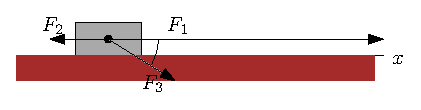
\includegraphics{img/disco.eps}
    \caption{Disco da hockey e vettori}
    \label{fig:hockeyevett}
  \end{figure}
  un disco da hockey si muove su una superficie ghiacciata priva di attrito lungo l'asse x in un moto unidirezzionale. La sua massa è $m=0.20kg$. Le forze $F_1$ ed $F_2$ di modulo rispettivamente 4.0N e 2.0N, agiscono lungo l'asse. Una terza forza $F_3$ di modulo 1.0N forma un angolo di $30^o$ rispetto all'asse x. In ciascuno dei tre casi qual è l'accelerazione del disco?
\end{es}
\begin{sol}
  In questo caso usuamo la seconda legge di Newton usando la formula della forza netta agente su un corpo, qui di forza c'è ne più di una quindi bisogna valutare le singole forze per poi calcolare l'accelerazione totale.
  \begin{eqnarray*}
    \vec{F}_{net}=m\vec{a} & \to{} & F_{net_x}=ma_x 
  \end{eqnarray*}
  Quindi se vogliamo trovare la forza di x dobbiamo fare una sommatoria:
  \begin{equation*}
    \sum F_x=ma_x
  \end{equation*}
  Da questo punto in poi dobbiamo calcolare $a_1x$ e $a_{2_1}$, visto che comunque il metodo migliore è procedere per punti con questo tipo di calcoli possiamo procedere nel seguente modo, creare un elenco ordinato e procedere in questo modo per evitare inutili disordini.
  \begin{enumerate}
  \item In primo luogo, conviene fare un veloce riepilogo delle variabili, quindi abbiamo 3 vettori/forze in gioco su questo corpo:
    \begin{equation*}
      \begin{cases}
        F_1=4.0N\\
        F_2=2.0N\\
        F_3=1.0N
      \end{cases}
    \end{equation*}
    con questo possiamo iniziare a lavorare sulle su $F_{1x}=ma_1x$ e $a_1x$.
    \begin{equation*}
      a_1x=\frac{F_{1x}}{m}=\frac{4N}{0.2kg}=20\frac{m}{s^2}
    \end{equation*}
  \item Visto che comunque $F_2$ ha vettorialmente un verso opposto a $F_1$ e quindi presenterà pure un segno algebrico opposto. Detto questo possiamo impostare la sommatoria $\sum F= F_{1x}-F_{2x}=ma_{2,1x}$
    \begin{equation*}
      a_{2_1}= \frac{F_{1x}-F_{2x}}{m}= \frac{4-2}{0.2}=\frac{2}{0.2}=10\frac{m}{s^2}
    \end{equation*}
  \item In extremis facciamo la somma vettoriale tra $F_2$ e $F_3$, quindi con la stessa formula usata prima possiamo calcolare anche questo caso\dots{}
    \begin{equation*}
      \sum F= -F_2x+F_2x=-2+1\cos30^o
    \end{equation*}
    $F_3$ ha un angolo di $30^o$ ed è contrassegnato con il simbolo $\uptheta$ e con questo abbiamo soddisfatto i requisiti posti dal testo.
  \end{enumerate}
\end{sol}
\clearpage
\begin{es}
  Un auto che slitta su una strada ghiacciata. Confrontiamo qui i tipici spazi di arresto necessari per fermarsi da una velocità iniziale di 10.0m/s su asfalto asciutto, fondo orizzontale ghiacciato e una strada gelata in discesa.
  \begin{figure}[ht!]
    \centering
    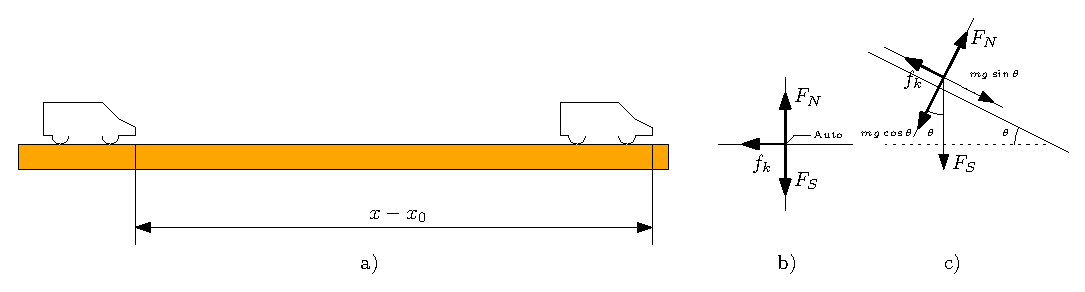
\includegraphics[scale=0.9]{img/auto.eps}
    \caption{Automobile su strada}
    \label{fig:autosust}
  \end{figure}
  \begin{tasks}
    \task Qual'è lo spazio d'arresto per un'auto su un piano orizzontale (\ref{fig:autosust}a) se il coefficiente di attrito è $\mu_k=0.60$, un valore tipico per pneumatici ordinari su asfalto asciutto? Trascuriamo gli effetti dell'aria, supponiamo che le ruote siano bloccate e che striscino sull'asfalto. Tracciamo l'asse $x$ nella direzione del moto.
    \task Quanto diventa lo spazio di frenata in condizioni di strada ghiacciata con $\mu_k=0,10$?
    \task Ora supponiamo che la macchina in frenata slitti su una discesa ghiacciata con inclinazione $\theta=6.00^o$ (una pendenza comune in montagna e in zonae collinose, pari a circa il 10.5\%). Quale sarebbe in tal caso lo spazio di arresto?
  \end{tasks}
\end{es}
\end{document}
